% ============================================================
% 第5章 Ordered Logit モデル：倒産距離 Z_lin の離散化と推定
% ============================================================

\chapter{Ordered Logit モデル：倒産距離 $Z_{\text{lin}}$ の離散化と推定}
\label{chap:ordered_logit}

\graphicspath{{figures/}}

本章では，第4章で導出した連続的倒産距離 $Z_{\text{lin}}$ を，
実証分析で扱う離散的な倒産ステージへと接続するための統計モデルとして，
Ordered Logit モデルを導入する。

倒産距離 $Z_{\text{lin}}$ は，企業価値プロセスと倒産閾値の関係を
連続的な尺度として表す理論モデルであるが，
実際の倒産データは「存続」「財務悪化」「撤退・吸収合併」「法的倒産」といった
離散的なステージとして観測される。
したがって，理論モデルで得られた連続量を，
実証分析で扱う離散カテゴリへと整合的に写像する枠組みが必要となる。

本章は，この写像を数学的に実現する Ordered Logit モデルの理論構造を提示し，
倒産距離 $Z_{\text{lin}}$ と潜在変数モデル $y^*$ の対応関係を明確化する章である。
まず，理論モデル・統計モデル・確率モデルがどのように連続的に接続されるかを
三層構造として整理し，Ordered Logit の導入位置づけを明確にする。


% ============================================================
% 5.1 理論モデル・統計モデル・確率モデルの三層構造
% ============================================================

\section{理論モデル・統計モデル・確率モデルの三層構造}
\label{sec:three_layer_structure}

本節では，本研究の倒産分析がどのように
「理論モデル（構造モデル）→ 統計モデル（潜在変数モデル）→ 確率モデル（Ordered Logit）」
という三層構造で接続されているかを整理する。

第4章で導出した線形倒産距離 $Z_{\text{lin}}$ は，
倒産距離 DD の一次近似\footnote{
ここでいう「一次近似」とは，Merton 型倒産距離の構造
（平均 $-$ 閾値）／不確実性を代表点の近傍で線形化したものであり，
Bharath \& Shumway（2008）の proxy DD の式そのものを展開したものではない。
}として倒産リスクの構造を表す決定論的指標である。
この連続的倒産距離を，観測可能データを用いて推定するためには，
潜在変数モデル $y^* = X\beta + \varepsilon$ に写像する必要がある。

さらに，潜在変数が複数の閾値 $\tau_k$ を跨ぐ構造を確率モデルへ接続することで，
Ordered Logit による離散的倒産ステージの確率的生成が実現される。

表 \ref{tab:theory_empirical_mapping} は，この対応関係を三つのステップとしてまとめたものである。

\begin{table}[H]
\centering
\caption{理論モデルと実証モデルの構造的対応（3ステップ）}
\label{tab:theory_empirical_mapping}
\begin{tabular}{p{3cm} p{6cm} p{6cm}}
\toprule
ステップ & 数式 & 役割 \\
\midrule
(1) 理論モデル（構造モデル） &
\(\displaystyle Z_{\text{lin}} = a\mu - b\sigma + cS - dThr\) &
倒産距離 DD の構造を一次近似した決定論的モデル \\

(2) 統計モデル（潜在変数モデル） &
\(\displaystyle y^* = X\beta + \varepsilon\) &
構造モデルを観測可能変数で推定するための統計的枠組み \\

(3) 確率モデル（Ordered Logit） &
\(\displaystyle \Pr(y=k)=\Lambda(\tau_k - X\beta)-\Lambda(\tau_{k-1}-X\beta)\) &
潜在変数を閾値で区切り，倒産ステージ確率を生成する \\
\bottomrule
\end{tabular}
\end{table}

図 \ref{fig:structural_mapping} に，理論モデル（\(Z_{\text{lin}}\)）と Ordered Logit の潜在変数モデルの構造的対応を示す。

\begin{figure}[H]
\centering
\begin{tikzpicture}[node distance=2.5cm]

\node[rectangle, draw, rounded corners, text width=7cm, align=center] (theory)
{\textbf{理論モデル（構造モデル）}\par
\(\displaystyle Z_{\text{lin}} = a\mu - b\sigma + cS - dThr\)
};

\node[rectangle, draw, rounded corners, text width=7cm, align=center, below=of theory] (latent)
{\textbf{統計モデル（潜在変数モデル）}\par
\(\displaystyle y^*_{i,t} = X_{i,t}\beta + \varepsilon_{i,t}\)\par
\(\displaystyle \varepsilon_{i,t} \sim \text{Logistic}(0,1)\)
};

\node[rectangle, draw, rounded corners, text width=8cm, align=center, below=of latent] (ordered)
{\textbf{確率モデル（Ordered Logit）}\par
閾値 \(\tau_k\) に基づくステージ確率\par
\(\displaystyle \Pr(y=k)=\Lambda(\tau_k - X\beta)-\Lambda(\tau_{k-1}-X\beta)\)
};

\draw[->, thick] (theory) -- node[midway, right]{構造的対応（写像）} (latent);
\draw[->, thick] (latent) -- node[midway, right]{ロジスティック分布により確率化} (ordered);

\end{tikzpicture}

\caption{理論モデル（\(Z_{\text{lin}}\)）と Ordered Logit の潜在変数モデルの構造的対応}
\label{fig:structural_mapping}
\end{figure}

% ============================================================
% 5.2 Ordered Logit の潜在変数構造
% ============================================================

\section{Ordered Logit の潜在変数構造}
\label{sec:ordered_latent_structure}

Ordered Logit モデルは，倒産ステージの背後に連続的な潜在変数
$y^*_{i,t}$ が存在すると仮定する潜在変数モデルである。
潜在変数は，企業の財務状態や市場環境など，倒産リスクに影響する要因を
線形に統合した上で，観測できないショックを加えたものである。

潜在変数モデルは次式で表される。


\[
y^*_{i,t}
=
X_{i,t}\beta + \varepsilon_{i,t},
\qquad
\varepsilon_{i,t} \sim \text{Logistic}(0,1)
\]



ここで，

\begin{itemize}
    \item $X_{i,t}$：倒産リスクに影響する観測可能な説明変数ベクトル  
    \item $\beta$：各説明変数の影響度を表す係数  
    \item $\varepsilon_{i,t}$：観測できないショック（ロジスティック分布に従う）
\end{itemize}

である。

ロジスティック分布を仮定することで，潜在変数が閾値を超える確率が
ロジスティック関数（ロジット確率）として表される。
この確率構造が Ordered Logit の基礎となる。

潜在変数の期待値は次式で与えられる。



\[
E[y^*_{i,t}] = X_{i,t}\beta
\]



これは，潜在倒産リスクの「中心」を表す量であり，
後述する線形倒産距離 $Z_{\text{lin}}$ と構造的に対応する。

潜在変数 $y^*$ は観測されないが，
その値が複数の閾値（cutpoints）をどこまで超えるかによって，
観測される倒産ステージが決定される。
この閾値構造については次節で詳述する。

% ============================================================
% 5.3 Ordered Logit の閾値構造（cutpoints）
% ============================================================

\section{Ordered Logit の閾値構造（cutpoints）}
\label{sec:ordered_cutpoints}

第3章では，倒産を「潜在変数が複数の閾値を跨ぐ現象」として捉える
Ordered Logit（順序ロジット）モデルの理論構造を示し，
倒産距離 DD の一次近似と閾値の役割がどのように接続されるかを整理した。
本節では，その理論的枠組みを踏まえつつ，
倒産が複数の段階と異なる「重さ（severity）」\footnote{
ここでいう「重さ（severity）」とは，倒産を単なる発生有無ではなく，
どの程度深刻な状態に至ったかという段階的な違いを表す概念である。
倒産研究では，破産・民事再生・撤退・吸収合併などの退出イベントは
企業にとって異なる経済的影響を持つため，
これらを区別せず二値化すると情報が大きく失われることが指摘されている
（Altman and Hotchkiss, 2006；Campbell, Hilscher and Szilagyi, 2008）。
Ordered Logit モデルは，こうした倒産の深刻度（severity）を
複数の段階として扱うことで，倒産プロセスの異質性をより精緻に捉えることができる。
}
を伴う現象であることを踏まえ，
従来の二値ロジットモデルでは新電力企業の倒産データを適切に扱えない理由を明確化し，
Ordered Logit を採用する必然性を示す。


\subsection*{二値ロジットの構造的限界：完全分離の問題}

新電力企業の倒産は極めて稀であり，
倒産＝1 の観測値が全体のごく一部に限られる。
このようなデータ構造では，従来の二値ロジットモデルにおいて
\textbf{完全分離（perfect separation）} が発生しやすい。
完全分離とは，説明変数の組み合わせが倒産企業と非倒産企業を
完全に識別してしまう状況を指す。
具体的には，ある説明変数の領域に倒産企業しか存在しない，
または非倒産企業しか存在しないという「完全な区分」が生じると，
ロジットモデルの尤度最大化において係数が無限大方向へ発散し，
有限の最尤推定量が存在しなくなる\footnote{
完全分離（perfect separation）とは，説明変数の組み合わせが
倒産＝1 と非倒産＝0 の観測値を完全に識別してしまう状況を指す。
具体的には，ある説明変数の領域に倒産企業しか存在しない，
または非倒産企業しか存在しないという「完全な区分」が生じると，
ロジットモデルの尤度最大化において係数が無限大方向へ発散し，
有限の最尤推定量が存在しなくなる。
ロジットモデルは


\[
\Pr(\text{Default}=1)=\Lambda(X\beta)
\]


という確率構造を持つため，倒産と非倒産が完全に分離されると，
$\Lambda(X\beta)$ を 0 または 1 に近づけるために
$X\beta$ を無限大にする必要が生じ，推定が数学的に不可能となる。
倒産企業が極端に少ない産業では典型的に発生する問題であり，
本研究の新電力企業データでも同様の現象が確認された。
}。

本研究でも，当初は倒産を二値（0/1）で定義したロジット推計を試みたが，
倒産企業が極めて少ないため，説明変数の組み合わせが
倒産と非倒産を完全に識別してしまい，最尤推定が発散する現象が確認された。
このため，倒産を二値で扱う枠組みでは，
新電力企業の倒産リスクを安定的に推定することができない。

\subsection*{倒産の段階性と Ordered Logit の必要性}

新電力企業の倒産プロセスは，単なる「倒産／非倒産」という二値ではなく，
財務悪化，撤退・吸収合併，法的倒産といった
\textbf{複数の段階を持つ現象}として観測される。
この段階性をモデル化するためには，
潜在変数 $y^*_{i,t}$ が複数の閾値（cutpoints）をどこまで超えるかによって
観測される倒産ステージが決定されるという構造が必要となる。

Ordered Logit モデルは，この「連続量 → 離散カテゴリ」の写像を
数学的に整合的に実現する標準的な枠組みである。
潜在変数 $y^*_{i,t}$ と倒産ステージの関係は次式で表される。



\[
\text{default\_stage}_{i,t} =
\begin{cases}
0 & (y^*_{i,t} < \tau_1) \\
1 & (\tau_1 \le y^*_{i,t} < \tau_2) \\
2 & (\tau_2 \le y^*_{i,t} < \tau_3) \\
3 & (\tau_3 \le y^*_{i,t})
\end{cases}
\]



ここで，

\begin{itemize}
    \item $\tau_1$：存続ステージと財務悪化ステージを分ける閾値  
    \item $\tau_2$：財務悪化ステージと撤退・吸収合併ステージを分ける閾値  
    \item $\tau_3$：撤退・吸収合併ステージと法的倒産ステージを分ける閾値  
\end{itemize}

である。

重要なのは，cutpoint（閾値）$\tau_k$ が研究者によって外生的に設定される値ではなく，
ロジット係数 $\beta$ と同様に尤度最大化（MLE）によって
\textbf{データから推定される内生的パラメータ}である点である。
つまり，閾値は「理論的に固定された境界」ではなく，
観測データとロジスティック分布の整合性を最も高めるように
推定される境界点である。

このため，潜在変数が特定の区間（例：$\tau_1 \le y^* < \tau_2$）に位置する場合でも，
Ordered Logit は 4 つのステージすべての確率を同時に計算する。
しかし，観測される倒産ステージは「最も確率が高いステージ」ではなく，
潜在変数がどの閾値区間に位置するかによって機械的に分類される。

\subsection*{本研究における実証的実装}

本研究では，観測可能性の制約から，
理論編で導入した 4 段階モデルを 3 段階モデルへ簡略化して推定する。
第4章で整形した財務データ・市場データを基礎として，
Ordered Logit 推定に必要な説明変数（debt\_ratio, asset\_growth, sigma）と
倒産ステージ（0・1・2）を付与し，
推定用パネルデータとして再構築した。

以上の理由から，Ordered Logit モデルは，
新電力企業の倒産リスクを複数段階の現象として扱うための
理論的・実証的に最も整合的な枠組みである。

% ============================================================
% 5.4 線形倒産距離 $Z_{\text{lin}}$ と潜在変数 $y^*$ の構造的対応
% ============================================================

\section{線形倒産距離 $Z_{\text{lin}}$ と潜在変数 $y^*$ の構造的対応}
\label{sec:zlin_y_mapping}

Bharath \& Shumway（2008）の倒産距離（proxy DD）は，
Merton 型モデルの「multiplicative → log → linear」という構造を保持したまま，
観測可能な財務データへ写像したものである。

本節では，第4章で導出した線形倒産距離 $Z_{\text{lin}}$ と，
Ordered Logit モデルの潜在変数 $y^*_{i,t}$ がどのように構造的に対応しているかを整理する。
この対応関係を明確にすることで，理論モデル（構造モデル）と統計モデル（潜在変数モデル）が
どのように連続的に接続されるかが理解できる。

% ------------------------------------------------------------
% (1) 記号と経済的意味の整理
% ------------------------------------------------------------

\subsection*{(1) 記号と経済的意味の整理}

まず，本研究で用いる主要な記号とその経済的意味を整理する。

\begin{table}[H]
\centering
\caption{潜在変数／倒産距離／閾値の記号整理}
\label{tab:latent_vars_unified}
\resizebox{\textwidth}{!}{%
\begin{tabular}{lll}
\hline
記号・呼称 & 数式上の定義 & 経済的意味 \\
\hline
$y^*$ & $X\beta$ & 潜在倒産リスク（連続値） \\
$Z_{\text{lin}}$ & $X\beta$ & 線形倒産距離（倒産閾値からの距離） \\
線形予測子 &
$X\beta = \beta_1 D + \beta_2 \mu + \beta_3 \sigma + \beta_4 S + \cdots$
& 倒産リスクに影響する要因の総合効果 \\
$\tau_k$ & cutpoints & 倒産ステージを区切る閾値 \\
$y$ & 0--3 & 観測される倒産ステージ \\
\hline
\end{tabular}
}
\end{table}

表~\ref{tab:latent_vars_unified} に示すように，
$X\beta$ は統計モデルと理論モデルの双方で現れるが，
その意味と役割は三者で明確に異なる。

\begin{itemize}
    \item \textbf{線形予測子 $X\beta$（統計モデル）}：  
    潜在変数の期待値（中心）を表す統計的概念。
    \item \textbf{潜在変数 $y^*$（確率モデル）}：  
    $X\beta$ に誤差項を加えた確率モデルの内部構造。
    \item \textbf{線形倒産距離 $Z_{\text{lin}}$（理論モデル）}：  
    倒産距離 DD を一次近似した決定論的指標。
\end{itemize}

数式の形は一致していても，意味は異なる点に注意が必要である。

% ------------------------------------------------------------
% (2) Zlin と y* の構造的対応
% ------------------------------------------------------------

\subsection*{(2) $Z_{\text{lin}}$ と $y^*$ の構造的対応}

Ordered Logit の潜在変数モデルは次式で表される。


\[
y^*_{i,t}
=
X_{i,t}\beta + \varepsilon_{i,t},
\qquad
\varepsilon_{i,t} \sim \text{Logistic}(0,1)
\]



ここで $X\beta$ は潜在倒産リスクの中心（期待値）を表す。

一方，第4章で導出した線形倒産距離は，


\[
Z_{\text{lin}} = a\mu - b\sigma + cS - dD
\]



であり，これは Ordered Logit の線形部分 $X\beta$ と同じ構造を持つ。

したがって，



\[
X\beta \;\;\longleftrightarrow\;\; Z_{\text{lin}}
\]



という対応関係が成立する。

さらに，潜在変数は



\[
y^*_{i,t} = Z_{\text{lin}} + \varepsilon_{i,t}
\]



と解釈でき，理論モデルで導出した倒産距離に観測できないショックを加えたものが
Ordered Logit の潜在変数である。

% ------------------------------------------------------------
% (3) 潜在変数の散らばりとロジスティック曲線
% ------------------------------------------------------------

\subsection*{(3) 潜在変数の散らばりとロジスティック曲線}

潜在変数 $y^*$ は誤差項によって上下に揺らぐ。
図~\ref{fig:latent_error_logistic} は，潜在変数の散らばりとロジスティック曲線の関係を示す。

\begin{figure}[H]
    \centering
    \begin{tikzpicture}
        \begin{axis}[
            width=0.9\linewidth,
            height=7cm,
            xmin=-4, xmax=4,
            ymin=-2, ymax=2,
            axis lines=middle,
            xlabel={潜在変数の理論値 $X\beta$},
            ylabel={潜在変数 $y^*$},
            samples=200
        ]
        \addplot[black, thick] {0.5*x};
        \addplot[
            only marks,
            mark=*,
            mark size=1.8pt,
            blue!60
        ]
        table {
            x   y
            -3.5 -2.0
            -2.5 -0.8
            -1.5 -0.3
            -0.5 -0.6
             0.5  0.7
             1.5 -0.9
             2.5  1.4
             3.5 -1.2
        };
        \addplot[
            red,
            thick,
            domain=-4:4
        ] {1/(1 + exp(-x))};
        \node at (axis cs:-3.5,0.8) [anchor=west, red] {ロジスティック曲線（確率）};
        \node at (axis cs:-3.5,-1.5) [anchor=west, blue!70] {潜在変数の散らばり（誤差項）};
        \node at (axis cs:2.2,1.2) [anchor=west, black] {$X\beta$（理論値）};
        \end{axis}
    \end{tikzpicture}
    \caption{潜在変数の散らばり（誤差項）とロジスティック曲線の関係}
    \label{fig:latent_error_logistic}
\end{figure}

青点は潜在変数のゆらぎを示す説明図であり，
赤線は倒産確率を表すロジスティック曲線である。

% ------------------------------------------------------------
% (4) 理論モデルから確率モデルへの橋渡し
% ------------------------------------------------------------

\subsection*{(4) 理論モデルから確率モデルへの橋渡し}

理論モデルで導出した倒産距離 $Z_{\text{lin}}$ は，
収益性 $\mu$，市場ショック感応度 $\sigma$，支援能力 $S$，倒産閾値 $\mathrm{Thr}$ を
線形に統合した決定論的指標である。

一方，Ordered Logit の潜在変数 $y^*_{i,t}$ は，
これらの要因を観測可能変数として推定し，
誤差項を加えることで確率モデルへと接続する統計的枠組みである。

したがって，



\[
y^*_{i,t} = Z_{\text{lin}} + \varepsilon_{i,t}
\]



という構造により，理論モデルで導出した倒産距離が，
Ordered Logit の確率モデルへと自然に橋渡しされる。

本研究の Ordered Logit モデルは，

\begin{quote}
\textbf{潜在変数 $y^*$ の線形部分を，理論モデルで導出した倒産距離 $Z_{\text{lin}}$ として具体化した実証モデル}
\end{quote}

として位置づけられる。





% ============================================================
% 5.5 Ordered Logit の確率式と MLE による推定
% ============================================================

\section{Ordered Logit の確率式と MLE による推定}
\label{sec:ordered_logit_mle}

前節までに，潜在変数 $y^*$ の構造と閾値（cutpoints）による倒産ステージの区分を示した。
本節では，Ordered Logit モデルがどのように倒産ステージの発生確率を計算し，
どのようにパラメータ（係数 $\beta$ と閾値 $\tau_k$）を推定するかを整理する。

% ------------------------------------------------------------
% (1) Ordered Logit の確率式
% ------------------------------------------------------------

\subsection*{(1) Ordered Logit の確率式}

潜在変数 $y^*$ が閾値 $\tau_k$ をどこまで超えるかによって，
観測される倒産ステージが決定されるため，
カテゴリ $k$ が観測される確率は次式で表される。


\[
\Pr(y = k)
=
\Lambda(\tau_k - X\beta)
-
\Lambda(\tau_{k-1} - X\beta)
\]


ここで，

\begin{itemize}
    \item $\Lambda(\cdot)$：ロジスティック分布の累積分布関数（CDF）
    \item $\tau_k$：カテゴリ $k$ の上側の閾値
    \item $\tau_{k-1}$：カテゴリ $k$ の下側の閾値
\end{itemize}

である。

この差分構造は，潜在変数モデル



\[
y^* = X\beta + \varepsilon, \qquad \varepsilon \sim \text{Logistic}(0,1)
\]



から直接導かれる。

ロジスティック分布の CDF は次式で表される。



\[
\Lambda(z) = \frac{1}{1 + e^{-z}}
\]



したがって，カテゴリ $k$ の発生確率は，
潜在変数が区間 $[\tau_{k-1}, \tau_k)$ に入る確率として計算される。

% ------------------------------------------------------------
% (2) 閾値（cutpoints）の推定
% ------------------------------------------------------------

\subsection*{(2) 閾値（cutpoints）の推定}

重要な点として，閾値 $\tau_k$ は研究者が外生的に設定する値ではなく，
係数 $\beta$ と同様に尤度最大化（MLE）によって
\textbf{データから推定される内生的パラメータ}である。

閾値は，潜在変数の連続スケールを複数カテゴリに区切る境界点として，
ロジスティック分布と観測データの整合性を最も高めるように推定される。

したがって，Ordered Logit は「閾値を推定するモデル」であり，
閾値は倒産ステージの境界を表す統計的な推定量である。

% ------------------------------------------------------------
% (3) 尤度関数と MLE
% ------------------------------------------------------------

\subsection*{(3) 尤度関数と MLE}

Ordered Logit の推定は，ロジスティック分布に基づく尤度関数を最大化する
数値最適化（MLE）によって行われる。

カテゴリ $k$ が観測されたときの尤度は式 \eqref{eq:ordered_prob} に基づき，



\[
L(\beta, \tau)
=
\prod_{i,t}
\left[
\Lambda(\tau_{y_{i,t}} - X_{i,t}\beta)
-
\Lambda(\tau_{y_{i,t}-1} - X_{i,t}\beta)
\right]
\]



となる。

非線形モデルであるため閉形式解は存在せず，
BFGS 法や Newton-Raphson 法などの数値アルゴリズムが内部で
cutpoints（閾値）を含む全パラメータを同時に推定する。

本研究では Python の \texttt{statsmodels} が内部で自動的に推定を行う。

% ------------------------------------------------------------
% (4) 潜在変数の値と倒産ステージ確率の関係
% ------------------------------------------------------------

\subsection*{(4) 潜在変数の値と倒産ステージ確率の関係}

潜在変数の値が右側へ移動するにつれて，
倒産ステージ確率がどのように入れ替わるかを図~\ref{fig:ordered_logit_stages} に示す。

\begin{figure}[H]
    \centering
    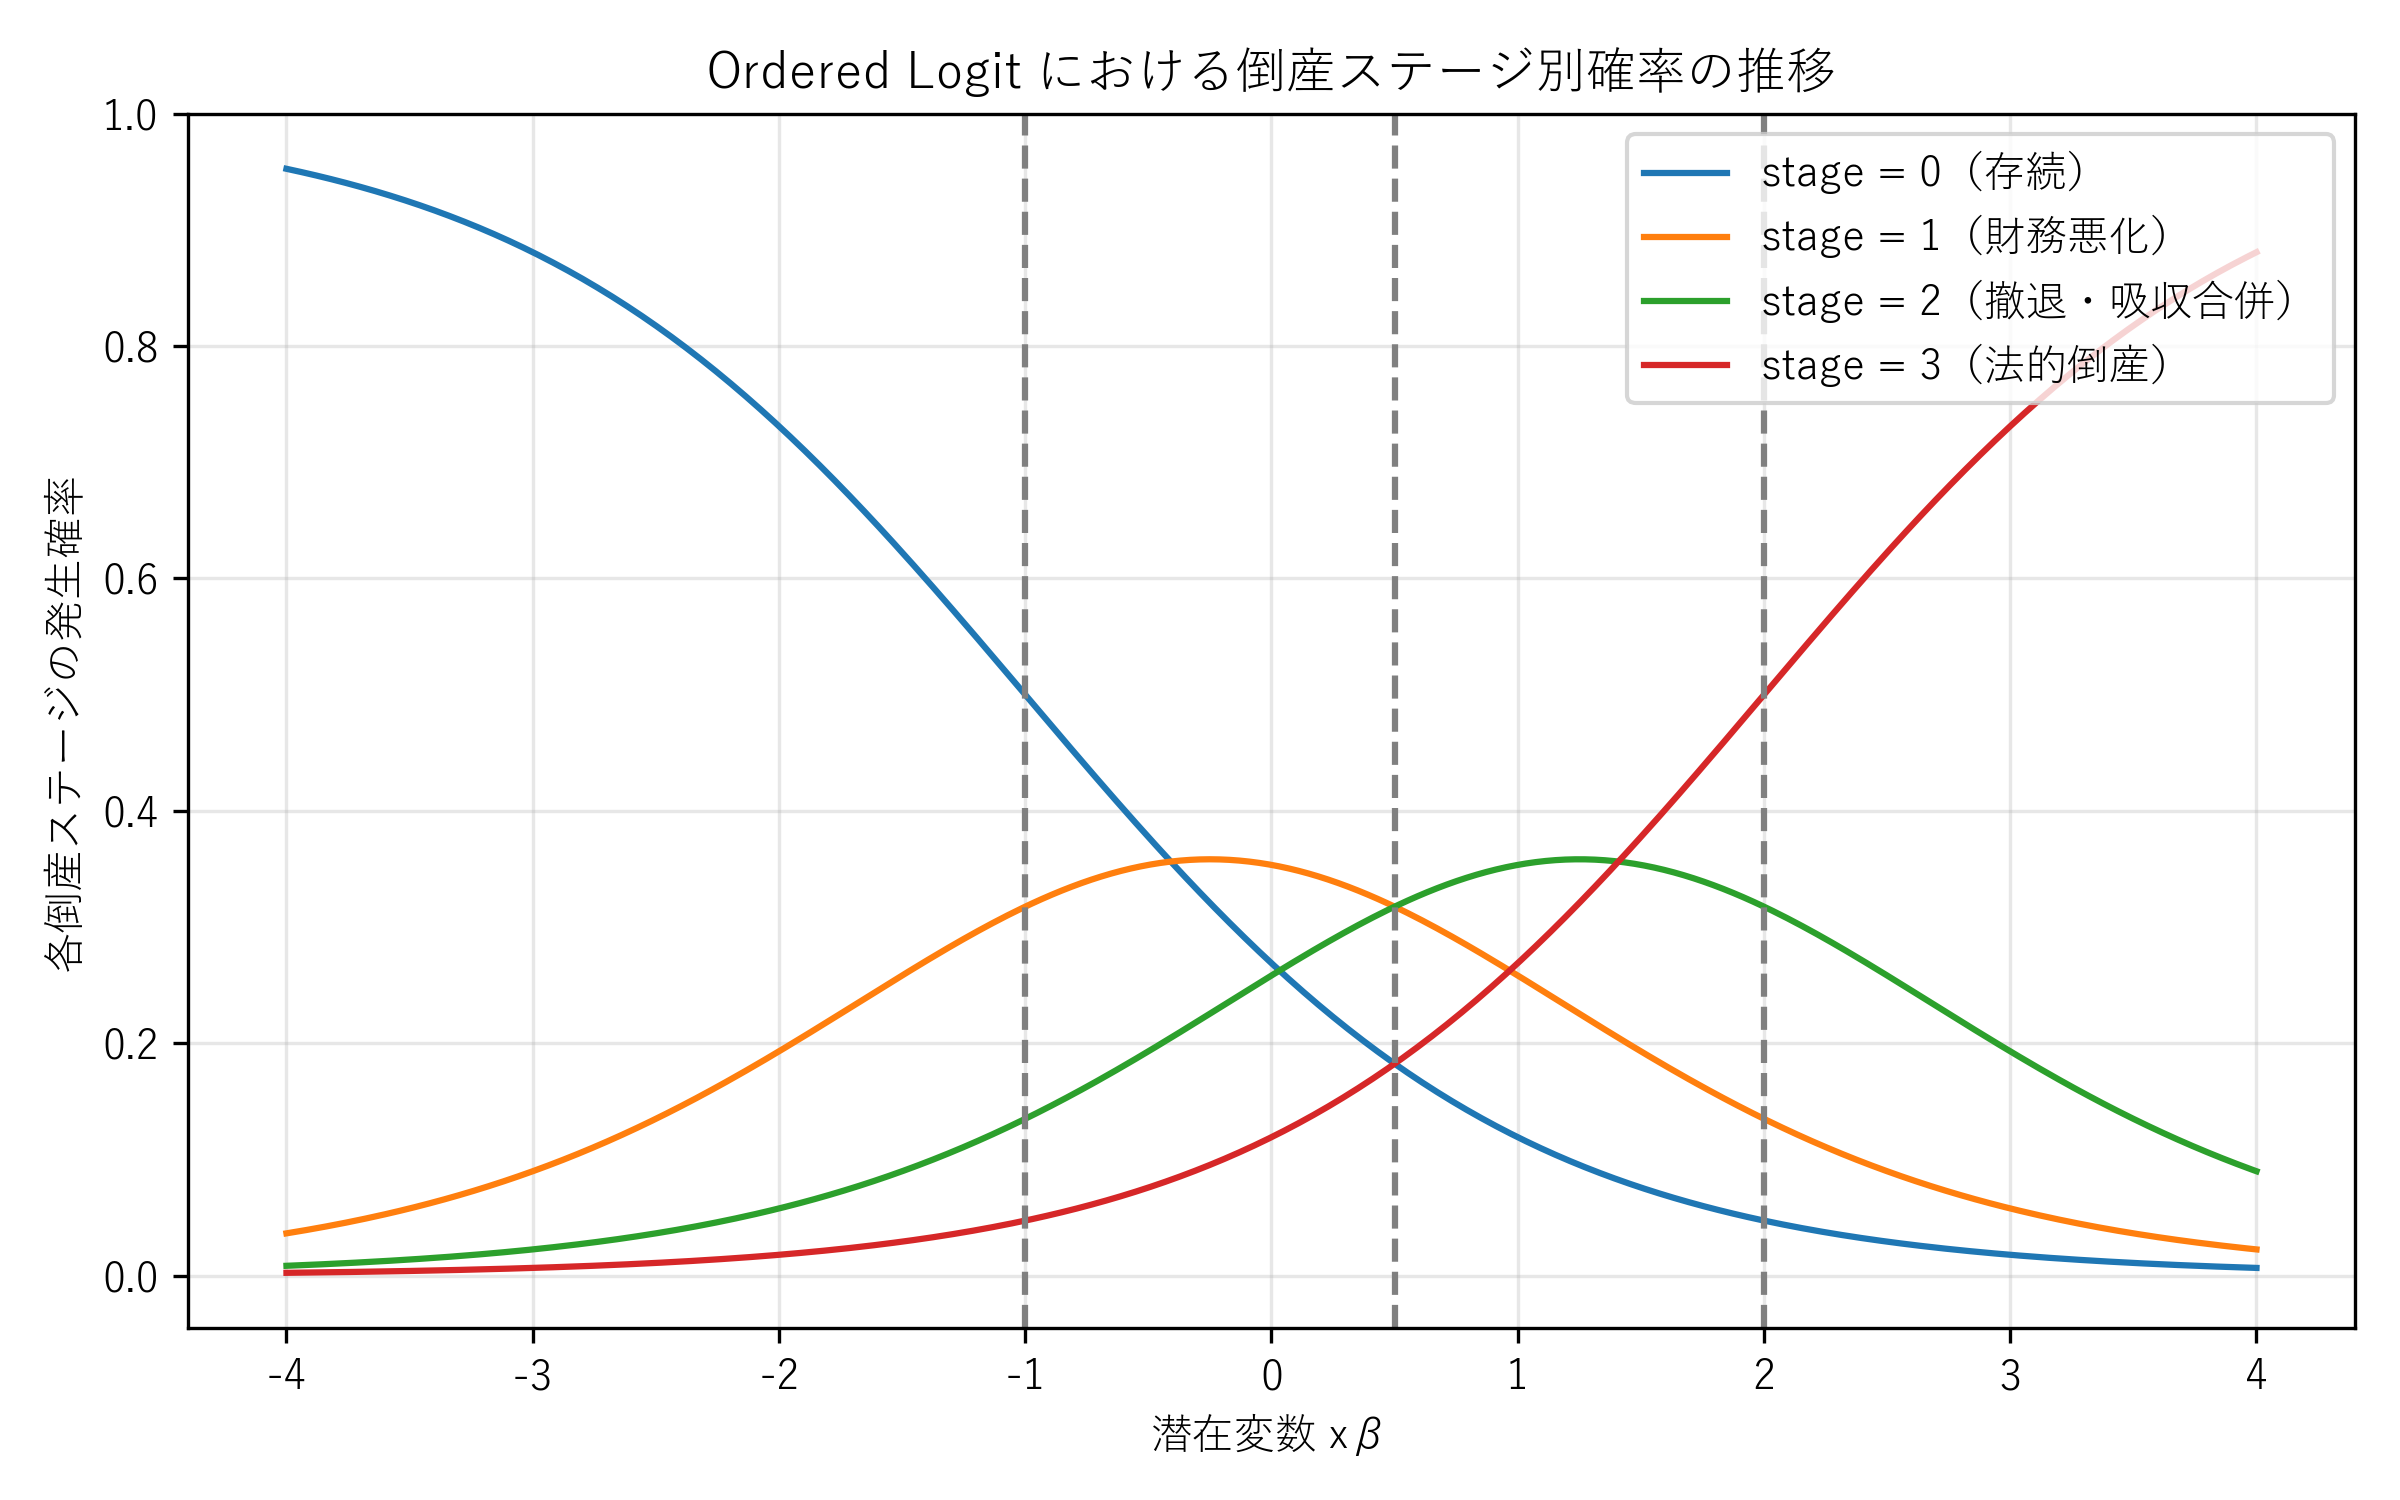
\includegraphics[width=0.85\linewidth]{ordered_logit_stages.png}
    \caption{潜在変数の値と倒産ステージ確率の関係}
    \label{fig:ordered_logit_stages}
\end{figure}

潜在変数が左側に位置する場合には存続ステージ（stage 0）の確率が高く，
右側へ進むにつれて，財務悪化（stage 1）→ 撤退・吸収合併（stage 2）
→ 法的倒産（stage 3）の順に確率が高まる。

この構造により，連続的な倒産リスクが離散的な倒産ステージへと
確率的に写像される Ordered Logit の特徴が明確になる。

% ============================================================
% 5.6 記号整理
% ============================================================

\section{記号整理}
\label{sec:notation}

本節では，本研究で用いる潜在変数モデル，線形倒産距離，閾値構造に関する
主要な記号を整理する。
Ordered Logit モデルは，潜在変数 $y^*$，線形予測子 $X\beta$，
閾値（cutpoints）$\tau_k$ の三つの構成要素によって成り立つため，
これらの記号の意味を明確にしておくことは重要である。

\begin{table}[H]
\centering
\caption{潜在変数／倒産距離／閾値の記号整理}
\label{tab:notation_summary}
\resizebox{\textwidth}{!}{%
\begin{tabular}{lll}
\hline
記号・呼称 & 数式上の定義 & 経済的意味 \\
\hline
$y^*$ & $X\beta + \varepsilon$ & 潜在倒産リスク（連続値） \\
$X\beta$ & $\beta_1 D + \beta_2 \mu + \beta_3 \sigma + \beta_4 S + \cdots$ & 潜在倒産リスクの中心（期待値） \\
$Z_{\text{lin}}$ & $a\mu - b\sigma + cS - dD$ & 倒産距離 DD の一次近似（構造モデル） \\
$\varepsilon$ & Logistic$(0,1)$ & 観測できないショック（誤差項） \\
$\tau_k$ & cutpoints & 倒産ステージを区切る閾値（推定される境界） \\
$y$ & 0--3 & 観測される倒産ステージ（離散カテゴリ） \\
\hline
\end{tabular}
}
\end{table}

表 \ref{tab:notation_summary} に示すように，
$X\beta$ は統計モデルと理論モデルの双方で現れるが，
その意味は異なる。

\begin{itemize}
    \item 統計モデルでは，$X\beta$ は潜在変数の期待値（中心）を表す。
    \item 理論モデルでは，$Z_{\text{lin}}$ が倒産距離 DD の一次近似として
          $X\beta$ と同じ線形構造を持つ。
    \item 確率モデルでは，$y^* = X\beta + \varepsilon$ が閾値 $\tau_k$ と比較され，
          観測される倒産ステージが決定される。
\end{itemize}

このように，数式の形は一致していても，
統計モデル・理論モデル・確率モデルの三者で役割が異なるため，
記号の整理は Ordered Logit の理解に不可欠である。

次節では，これらの記号を用いて，
線形倒産距離 $Z_{\text{lin}}$ と潜在変数 $y^*$ の構造的対応を詳細に示す。

% ============================================================
% 5.7 本章のまとめ
% ============================================================

\section{本章のまとめ}
\label{sec:ordered_logit_summary}

本章では，第4章で導出した連続的倒産距離 $Z_{\text{lin}}$ を，
実証分析で扱う離散的倒産ステージへと接続するための統計モデルとして
Ordered Logit モデルを体系的に整理した。

まず，理論モデル（構造モデル），統計モデル（潜在変数モデル），
確率モデル（Ordered Logit）の三層構造を提示し，
連続的倒産距離を離散的倒産ステージへと写像するための
概念的枠組みを明確にした。

次に，潜在変数 $y^*$ の構造と閾値（cutpoints）による区分を示し，
潜在倒産リスクがどのように離散カテゴリとして観測されるかを整理した。
閾値 $\tau_k$ は外生的に設定される境界ではなく，
係数 $\beta$ と同様に尤度最大化（MLE）によって推定される
内生的パラメータである点を強調した。

さらに，線形倒産距離 $Z_{\text{lin}}$ と潜在変数 $y^*$ の構造的対応を示し，
理論モデルで導出した倒産距離が，
潜在変数モデルの線形部分 $X\beta$ と同じ構造を持つことを明らかにした。
この対応関係により，理論モデルで得られた倒産距離が，
Ordered Logit の確率モデルへと自然に橋渡しされることを示した。

最後に，Ordered Logit の確率式と MLE による推定方法を整理し，
潜在変数の値が右側へ移動するにつれて倒産ステージ確率がどのように変化するかを
図示した。

以上の議論により，本研究の Ordered Logit モデルは，

\begin{quote}
\textbf{理論モデルで導出した倒産距離 $Z_{\text{lin}}$ を，
潜在変数モデルと閾値構造を用いて離散的倒産ステージへと写像する確率モデル}
\end{quote}

として位置づけられる。

次章では，本章で整理した Ordered Logit モデルを用いて，
英国新電力企業の倒産ステージを実証的に推定し，
倒産距離 $Z_{\text{lin}}$ の構造が実際の倒産データとどのように整合するかを検証する。
